\documentclass[12pt]{kiarticle} % You can learn about my document class "kiarticle" and install it to your device by following the link: https://github.com/Kiarendil/toolkitex
\graphicspath{{pictures/}}
\DeclareGraphicsExtensions{.pdf,.png,.jpg,.eps}
%%%
\pagestyle{fancy}
\fancyhf{}
%\renewcommand{\headrulewidth}{ 0.1mm }
\renewcommand{\footrulewidth}{ .0em }
\fancyfoot[C]{\texttt{\textemdash~\thepage~\textemdash}}
\fancyhead[L]{Лабораторная работа № 3.3.4 \hfil}
\fancyhead[R]{\hfil Иванов Кирилл, 625 группа }
\usepackage{multirow} % Слияние строк в таблице
\newcommand
{\un}[1]
{\ensuremath{\text{#1}}}
\newcommand{\eds}{\ensuremath{ \mathscr{E}}}
\usepackage{tikz}
%%% Работа с таблицами
\usepackage{array,tabularx,tabulary,booktabs} % Дополнительная работа с таблицами
\usepackage{longtable}  % Длинные таблицы
\usepackage{multirow} % Слияние строк в таблице

\begin{document}
	
	\begin{titlepage}
		\begin{center}
			\large 	Московский физико-технический институт \\
			Факультет общей и прикладной физики \\
			\vspace{0.2cm}
			
			\vspace{4.5cm}
			Лабораторная работа № 3.3.4 \\ \vspace{0.2cm}
			\large (Общая физика: электричество и магнетизм) \\ \vspace{0.2cm}
			\LARGE \textbf{Эффект Холла в полупроводниках}
		\end{center}
		\vspace{2.3cm} \large
		
		\begin{center}
			Работу выполнил: \\
			Иванов Кирилл,
			625 группа
			\vspace{10mm}		
			
		\end{center}
		
		\begin{center} \vspace{60mm}
			г. Долгопрудный \\
			2017 год
		\end{center}
	\end{titlepage}
	
	
	\paragraph*{Цель работы:} измерение подвижности и концентрации носителей заряда в полупроводниках.
	
	\paragraph*{Оборудование:} электромагнит с источником питания, батарейка, амперметр, реостат, цифровой вольтметр, милливеберметр, образцы легированного германия.
	
	\section{Теоретическая справка}
	Суть эффекта Холла состоит в следующем. Пусть через однородную пластину металла вдоль оси $x$ течет ток $I$ (рис. 1).
	
	\begin{wrapfigure}{l}{0.6\textwidth}
		\vspace{-20pt}
		\begin{center}
			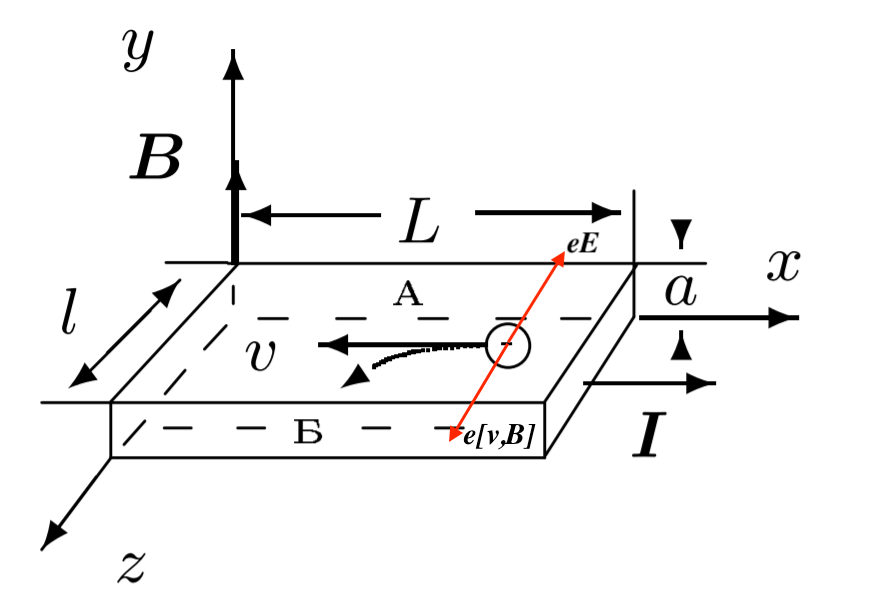
\includegraphics[width=0.7\linewidth]{Holl1.png}
			\label{fig:sdfsafd}
		\end{center}
		\vspace{-20pt}
		\caption{Образец с током в магнитном поле}
	\end{wrapfigure}

	Если эту пластину поместить в магнитное поле, направленное по оси y, то между гранями А и Б появляется разность потенциалов. 
	
	В самом деле, на электрон (для простоты рассматриваем один тип носителей), движущийся со средней скоростью $\langle \vec{v} \rangle$ в электромагнитном поле, действует сила Лоренца:
	
	$$\vec{F}_{л} = -e\vec{E}-e \langle \vec{v} \rangle \times \vec{B},$$
	
	где $e$- абсолютный заряд электрона, $\vec{E}$ - напряженность электрического поля, $\vec{B}$ - индукция магнитного поля.
	
	В проекции на ось $z$ получаем
	
	$$ F_{B}=e | \langle {v_{x}} \rangle | B.$$
	
	Под действием этой силы электроны отклоняются к грани Б, заряжая ее отрицательно. На грани А накапливаются нескомпенсированные положительные заряды. Это приводит к возникновению электрического поля $E_{z}$, направленного от А к Б, которое действует на электроны с силой $F_{E}=eE_{z}$. В установившемся режиме $F_{E}=F_{B}$, поэтому накопление электрических зарядов на боковых гранях пластины прекращается. Отсюда
	
	$$ E_{z}=| \langle {v_{x}} \rangle | B.$$
	
	С этим полем связана разность потенциалов $$U_{AБ}=E_{z}l=| \langle {v_{x}} \rangle | Bl.$$
	
	В этом и состоит эффект Холла.
	
	\
	
	Замечая, что сила тока
	
	$$ I=ne| \langle {v_{x}} \rangle |la,$$
	
	найдем ЭДС Холла:
	
\begin{equation}\label{Rx}
	\mathscr{E}_{X}=U_{AБ}=\dfrac{IB}{nea}=R_{X}\dfrac{IB}{a}
\end{equation}
	
	Константа $R_{X}=\dfrac{1}{ne}$ называется постоянной Холла.
	
	В полупроводниках, когда вклад в проводимость обусловлен и электронами и дырками, выражение для постоянной Холла имеет более сложный вид:
	
	$$R_{X}=\dfrac{nb^{2}_{e}-pb^{2}_{p}}{e(nb_{e}+pb_{p})^{2}},$$
	
	где $n$ и $p$ - концентрации электронов и дырок, $b_{e}$ $b_{p}$ - их подвижности.
	
	\section{Экспериментальная установка.}
	Схема экспериментальной установки показана на рис. 2.
	
	\begin{figure}[h!]
		\centering
		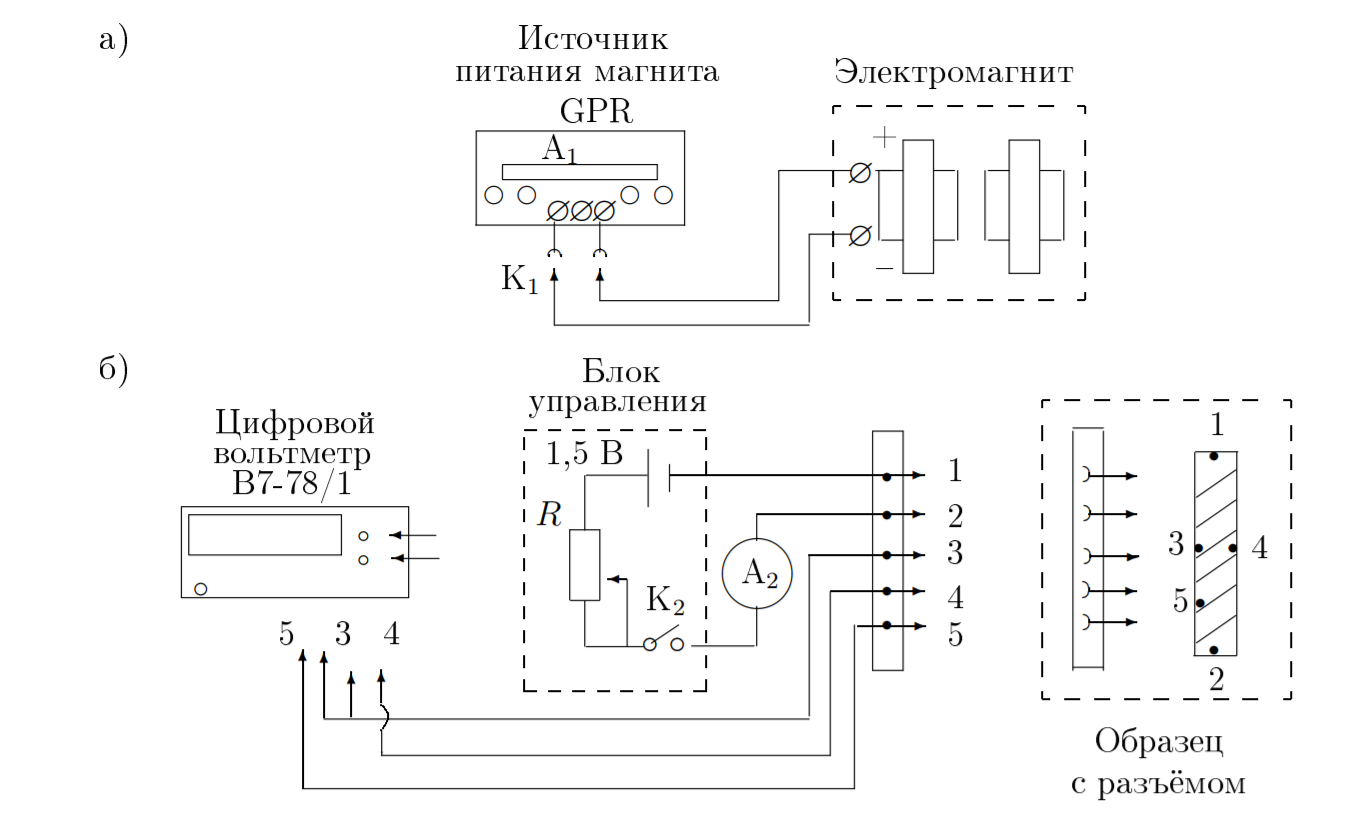
\includegraphics[width=\linewidth]{Holl2}
		\caption{Схема установки для исследования эффекта Холла в полупроводниках}
		\label{fig:Holl2}
	\end{figure}
  
  	В зазоре электромагнита (рис. 1а) создаётся постоянное магнитное поле, величину которого можно менять с помощью регуляторов источника питания. Ток измеряется амперметром источника питания $A_{1}$. Разъем $K_{1}$ позволяет менять направление тока в обмотках электромагнита.
  
  	Образец из легированного германия, смонтированный в специальном держателе (рис. 1б), подключается к батарее. При замыкании ключа $K_{2}$ вдоль длинной стороны образца течет ток, величина которого регулируется реостатом $R$ и измеряется миллиамперметром $А_{2}$.
  	
  	В образце с током, помещённом в зазор электромагнита, между контактами 3 и 4 возникает разность потенциалов $U_{34}$, которая измеряется с помощью цифрового вольтметра.
  	
  	Контакты 3 и 4 вследствие неточности подпайки не всегда лежат на одной
  	эквипотенциали, и тогда напряжение между ними связано не только с эффектом
  	Холла, но и с омическим падением напряжения, вызванным протеканием основного тока через образец.
  	
  	Измеряемая разность потенциалов при одном направлении
  	магнитного поля равна сумме ЭДС Холла и омического падения напряжения, а
  	при другом  их разности. В этом случае ЭДС Холла $\mathscr{E}_{X}$ может быть определена как половина алгебраической разности показаний вольтметра, полученных для
  	двух противоположных направлений магнитного поля в зазоре.
  	
  	Можно исключить влияние омического падения напряжения иначе, если при каждом токе через образец измерять напряжение между точками 3 и 4 в отсутствие магнитного поля. При фиксированном токе через образец это дополнительное к ЭДС Холла напряжение $U_{0}$ остается неизменным. От него следует (с учетом
  	знака) отсчитывать величину ЭДС Холла: 
  	
  	$$\mathscr{E}_{X} = U_{34} \pm U_{0}$$. 
  	
  	При таком способе измерения нет необходимости проводить повторные измерения с противоположным направлением магнитного поля.
  	
  	
  	По знаку $\mathscr{E}_{X}$ можно определить характер проводимости - электронный или дырочный. Для этого необходимо знать направление тока в образце и направление
  	магнитного поля.
  	
  	Измерив ток $I$ в образце и напряжение $U_{35}$ между контактами 3 и 5 в отсутствие магнитного поля, можно, зная параметры образца, рассчитать проводимость материала образца по формуле:
  	
  \begin{equation}\label{sigma}
  	\sigma=\dfrac{IL_{35}}{U_{35}al}
  \end{equation}
  	
  	где $L_{35}$ - расстояние между контактами 3 и 5, $a$ - толщина образца, $l$ - его ширина.
  	
  	\section{Ход работы}
  	
  	\begin{enumerate}
  	\item Запишем данные установки:
  	
  	$a=2,2 \; мм,$ $L_{35}=6,0 \;мм,$ $l=7,0 \;мм,$ $SN=75 \;см^{2}\cdot вит$ - площадь сечения контура катушки на число витков в ней.
  	
  	\item Настроим приборы согласно инструкции.
  	
  	\item Запишем предельное значение тока через электромагнит:
  	
  	$$ I_{max}=2,13 \; А.$$
  	
  	\item Исследуем зависимость потока $ \Phi $ магнитного поля в зазоре электромагнита от тока через обмотки магнита. Данные занесём в табл. 1.
  	
  	Индукцию $B$ найдем по формуле
  	
  \begin{equation}\label{}
  	B=\dfrac{\Delta Ф}{SN},
  \end{equation}
  	
  	где $\Delta Ф = Ф - Ф_{0}$ - разность между начальным и конечным значением потока вектора индукции, который пронизывал пробную катушку, находившуюся в зазоре электромагнита.
  	
  	
\begin{figure}[h!]
	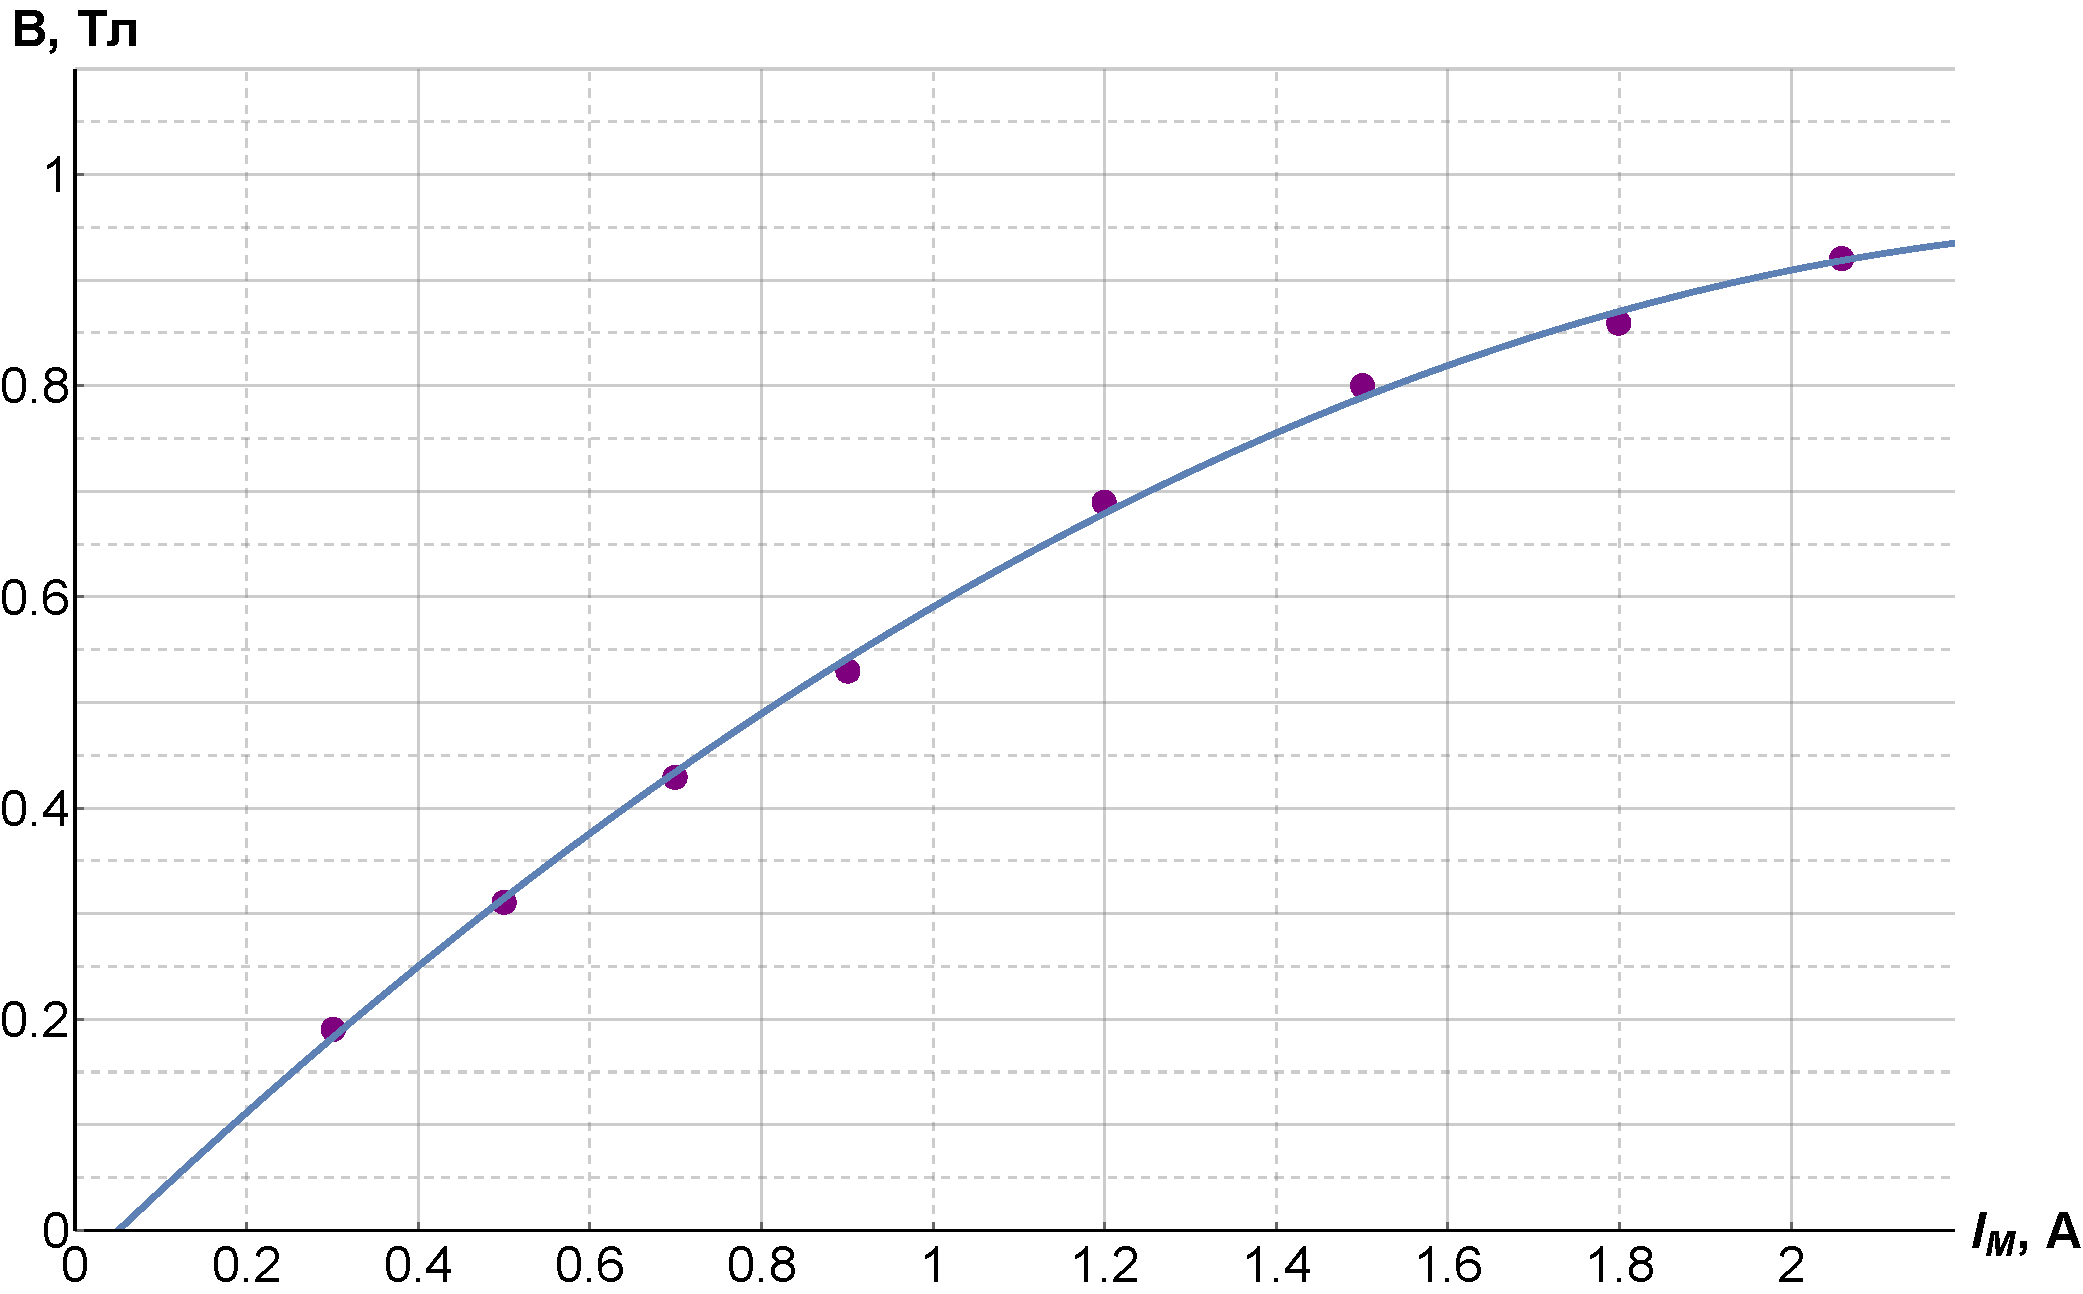
\includegraphics[scale=0.5]{B.pdf}
	\caption{График зависимости $ B(I_M) $}
\end{figure}
  	
  		
  	
  		\begin{table}[]
  			\caption{Зависимость $B(I_{м})$}
  		\begin{center}
  		\begin{tabular}{|c|c|c|c|c|c|} 
  			\hline 
  			№ &  $I_{м}$, A &  $Ф_{0}$, мВб & $Ф$, мВб & $\Delta Ф$, мВб & $B, Тл$  \\ 	\hline
  			
  			1 & 0,30 & 2 & 3,4 & 1,4 & 0,19 \\
  			2 & 0,50 & 2 & 4,3 & 2,3 & 0,31 \\
  			3 & 0,70 & 2 & 5,2 & 3,2 & 0,43 \\
  			4 & 0,90 & 2 & 6,0 & 4,0 & 0,53 \\
  			5 & 1,20 & 2 & 7,2 & 5,2 & 0,69 \\
  			6 & 1,50 & 2 & 8,0 & 6,0 & 0,80\\
  			7 & 1,80 & 2 & 8,5 & 6,5 & 0,86\\
  			8 & 2,06 & 2 & 8,9 & 6,9 & 0,92\\
  			\hline
  			
  		\end{tabular}
  	\end{center}
  \end{table}

  	По этим данным построим график зависимости $B=B(I_{M})$ (рис. 3).
  	
  	\item Снимем зависимость $U_{34}(I_{м})$ различных токах через образец (табл. 2). А именно, он изменяется от 0,23 до 1,07 мА. При этом в отсутствие магнитного поля вольтметр покажет напряжение $U_{0}$. Результаты занесём в таблицу 2, подписывая сверху $ I, U_0 $  в мА и мкВ соответственно. В последнем опыте изменим направление магнитного поля.  
  
  \begin{table}[h!]
  	\centering
  	\caption{Результаты измерений $ U_{34} $}
  	\begin{tabularx}{\textwidth}{|c|c|c|c|c|c|c|c|c|c|}
  		\hline
  		\multirow{3}{*}{$ N $} & \multirow{3}{*}{$ I_M, A $} & 
  		$I, \; U_0 $ &
  			$I, \;U_0 $ &
  			$I, \;U_0 $ &
  		$I, \;U_0 $ &
  		$I, \;U_0 $ & 
  		$I, \;U_0 $ &
  		$I, \;U_0 $ &
  			$I, \;U_0 $ 
  		\\
  		& &
  		 $0,22,  \;46$ &
  		$ 0,35,  \;72 $ &
  		   $  0,50, \;102$ &
  		     $  0,60,  \;123$ &
  		     $ 0,70,  \;145$ & 
  		      $ 0,85, \; 175$ &
  		      $  1,07,  \;220 $  &
  		      $ 1,07,\; 220 $
  		       \\
  		       \cline{3-10}
  		       & & \multicolumn{8}{|c|}{$ U_{34}, \; мкВ $} \\
  		       \hline
  		 1& 0.1& 38 & 62 & 88 & 107 & 125 & 150 & 191 & 268 \\
  		2 & 0.3 & 27 & 41 & 57 & 69 & 83 & 100 & 124 & 334 \\
  		3 & 0.6 & 8 & 10 & 13 & 17 & 18 & 23 & 32 & 432 \\
  		4 & 0.9 & -9 & -15 & -20 & -28 & -28 & -34 & -42 & 517 \\
  		5 & 1.2 & -22 & -34 & -49 & -60 & -68 & -81 & -104 & 582 \\
  		6 & 1.5 & -30 & -48 & -67 & -82 & -94 & -114 & -144 & 629 \\
  		7 & 1.8 & -36 & -56 & -89 & -96 & -112 & -135 & -169 & 658 \\
  		8 & 2.1 & -40 & -62 & -88 & -106 & -123 & -146 & -184 & 674 \\
  		\hline
  	\end{tabularx}
  	\label{resU}% 
  \end{table}% 
  
  Рассчитаем ЭДС Холла $ \eds_X $ по формуле и занесем результаты в таблицу 3:
  
  \begin{equation}\label{}
  \eds_X = U_{34} - U_0
  \end{equation}
  
    \begin{table}[h!]
  	\centering
  	\caption{Результаты измерений $ \eds_X $}
  	\begin{tabularx}{\textwidth}{|c|c|c|c|c|c|c|c|c|c|}
  		\hline
  		\multirow{3}{*}{$ N $} & \multirow{3}{*}{$ I_M, A $} & 
  		$I, \; U_0 $ &
  		$I, \;U_0 $ &
  		$I, \;U_0 $ &
  		$I, \;U_0 $ &
  		$I, \;U_0 $ & 
  		$I, \;U_0 $ &
  		$I, \;U_0 $ &
  		$I, \;U_0 $ 
  		\\
  		& &
  		$0,22,  \;46$ &
  		$ 0,35,  \;72 $ &
  		$  0,50, \;102$ &
  		$  0,60,  \;123$ &
  		$ 0,70,  \;145$ & 
  		$ 0,85, \; 175$ &
  		$  1,07,  \;220 $  &
  		$ 1,07,\; 220 $
  		\\
  		\cline{3-10}
  		& & \multicolumn{8}{|c|}{$ \eds_X, \; мкВ $} \\
  		\hline
  	1 & 0.1 & -8 & -10 & -14 & -16 & -20 & -25 & -29 & -28 \\
  	2 & 0.3 & -19 & -31 & -45 & -54 & -62 & -75 & -96 & -94 \\
  	3 & 0.6 & -38 & -62 & -89 & -106 & -127 & -152 & -188 & -192 \\
  	4 & 0.9 & -55 & -87 & -122 & -151 & -173 & -209 & -262 & -277 \\
  	5 & 1.2 & -68 & -106 & -151 & -183 & -213 & -256 & -324 & -342 \\
  	6 & 1.5 & -76 & -120 & -169 & -205 & -239 & -289 & -364 & -389 \\
  	7 & 1.8 & -82 & -128 & -191 & -219 & -257 & -310 & -389 & -418 \\
  	8 & 2.1 & -86 & -134 & -190 & -229 & -268 & -321 & -404 & -434 \\
  		\hline
  	\end{tabularx}
  	\label{resF}% 
  \end{table}% 
  
  Теперь вычислим $ R_X $ из формулы \eqref{Rx}:
  
  \begin{equation}\label{}
  R_X = \dfrac{a\eds_X}{BI}
  \end{equation}
  
  Результаты сведем в таблицу 4:
  
  
      \begin{table}[h!]
  	\centering
  	\caption{Результаты измерений $ R_X $}
  	\begin{tabularx}{\textwidth}{|c|c|c|c|c|c|c|c|c|c|}
  		\hline
  		\multirow{3}{*}{$ N $} & \multirow{3}{*}{$ B, Тл$} & 
  		$I, \; U_0 $ &
  		$I, \;U_0 $ &
  		$I, \;U_0 $ &
  		$I, \;U_0 $ &
  		$I, \;U_0 $ & 
  		$I, \;U_0 $ &
  		$I, \;U_0 $ &
  		$I, \;U_0 $ 
  		\\
  		& &
  		$0,22,  \;46$ &
  		$ 0,35,  \;72 $ &
  		$  0,50, \;102$ &
  		$  0,60,  \;123$ &
  		$ 0,70,  \;145$ & 
  		$ 0,85, \; 175$ &
  		$  1,07,  \;220 $  &
  		$ 1,07,\; 220 $
  		\\
  		\cline{3-10}
  		& & \multicolumn{8}{|c|}{$ R_X \x 10^{-4}, \dfrac{м^3}{Кл} $} \\
  		\hline
  		1 & 0.17 & 4.7 & 3.7 & 3.6 & 3.5 & 3.7 & 3.8 & 3.5 & 3.4 \\
  		2 & 0.19 & 10.0 & 10.3 & 10.4 & 10.4 & 10.3 & 10.2 & 10.4 & 10.2 \\
  		3 & 0.37 & 10.3 & 10.5 & 10.6 & 10.5 & 10.8 & 10.6 & 10.4 & 10.7 \\
  		4 & 0.53 & 10.4 & 10.3 & 10.1 & 10.4 & 10.3 & 10.2 & 10.2 & 10.7 \\
  		5 & 0.69 & 9.9 & 9.7 & 9.6 & 9.7 & 9.7 & 9.6 & 9.7 & 10.2 \\
  		6 & 0.8 & 9.5 & 9.4 & 9.3 & 9.4 & 9.4 & 9.4 & 9.4 & 10.0 \\
  		7 & 0.86 & 9.5 & 9.4 & 9.8 & 9.3 & 9.4 & 9.3 & 9.3 & 10.0 \\
  		8 & 0.92 & 9.3 & 9.2 & 9.1 & 9.1 & 9.2 & 9.0 & 9.0 & 9.7 \\
  		\hline
  	\end{tabularx}
  	\label{resR}% 
  \end{table}% 

  
  \item 
  Теперь посчитаем для наших $ R_X $, начиная со вторых значений, истинное среднее, вычисляя погрешность через коэффициент Стьюдента, равный $ A = 2 $.
  
  \begin{equation}\label{}
  R_X = R_{ср} \pm A\dfrac{\sigma}{\sqrt{N}}
  \end{equation}  
  
  $ R_{ср} \approx 9,9 \x 10^{-4}, \dfrac{м^3}{Кл} $ --- среднее арифметическое, $ \sigma \approx 0,5 $ --- среднеквадратичное отклонение,$ N = 56. $
  Отсюда 
  
  \begin{equation}\label{}
  R_X = (9,9 \pm 0,2) \x 10^{-4}, \dfrac{м^3}{Кл}
  \end{equation}
  
 \item

Определим, что наши частицы движутся к клемме №4 образца. Зная направление магнитного поля в электромагните и тока через образец, мы определяем, что наши частицы заряжены отрицательно, т.е. являются электронами.
  
  \item 
  
  Теперь определим концентрацию электронов:
 
\begin{equation}\label{}
   n = \dfrac{1}{R_Xe} \pm \dfrac{1}{R_Xe} \dfrac{\sigma_{R_X}}{R_X} \approx (6,3 \pm 0,1) \x 10^{21} \dfrac{1}{м^3}
\end{equation}

\item При токе через образец $ I = 1 $ мА по формуле \eqref{sigma} посчитаем удельную проводимость:

\begin{equation}\label{}
\sigma \approx (80,8 \pm 0,6) \x \dfrac{1}{Ом \x м}
\end{equation}

\item

По формуле посчитаем подвижность электронов: 

\begin{equation}\label{}
b = \dfrac{\sigma}{en} \approx (797 \pm 11) \dfrac{см^2}{В\x с}
\end{equation}

\item 

Построим итоговую таблицу:

\begin{tabular}{|c|c|c|c|c|}
	\hline 
	$ R_X, $ & \multirow{2}{*}{Знак носителей} & $ n, $ &$  \sigma, $ & $ b, $ \\ 

	$ 10^{-4} \; м^3/Кл $ &  & $ 10^{21}, м^{-3} $ & $ Ом^{-1} \x м^{-1}  $&$  см^2/ В \x с $ \\ 
	\hline 
$ 	9,9 \pm 0,2  $ & $ -  $ & $ 6,3 \pm 0,1  $ & $ 80,8 \pm 0,6 $ & $ 797 \pm 11 $ \\ 
	\hline 
\end{tabular} 

\section{Вывод}

Мы изучили явление эффекта Холла в полупроводниках, измерили для нашего образца (Германий) такие величины как постоянная Холла, концентрацию электронов, удельную проводимость и подвижность электронов.

Допуская существование добавок в материале образца, результаты вполне соответствуют табличным. 

  
 	 
  	
\end{enumerate}
\end{document}